\documentclass[portrait]{ppgcaposter}

\newcommand{\FFCLRP}{Faculdade de Filosofia, Ci\^{e}ncias e Letras de Ribeir\~{a}o Preto}

%%%% INSIRA O TITULO AQUI
\def\titulo{Lorem ipsum dolor}

\begin{document}
\printheader
\begin{center}
  %% TITLE
  \textbf{\bf\huge\color{NavyBlue}\titulo\\[.5cm]}
  
  %% AUTHORS
  
  \LARGE  A. Turing$^{1*}$, C.F. Gau{\ss}$^1$, J. von Neumann$^1$, R.P. Feynman$^2$\\[0.3cm]
  \Large Programa de Pós-Graduação em Computação Aplicada\\[0.3cm]
  \Large $^1$Departamento de Computação e Matemática, \FFCLRP--USP\\[0.3cm]
  $^2$Departamento de Física, \FFCLRP--USP\\[0.2cm]
  \large {\tt$^*$turing@dcm.ffclrp.usp.br}

 \end{center}

\vspace{2cm}

%%%% Retire os comentários se houver RESUMO %%%%
%%%%
% \color{Navy}
% \begin{abstract}

%   Te ancillae contentiones vix, ad partiendo patrioque inciderint
%   eum. Mea porro regione ex. Case iuvaret ocurreret quo at, legere
%   malorum indoctum cu his. Eros ubique mel in. At duo partem vidisse
%   intellegam. Equidem detraxit has ea. Phasellus imperdiet, tortor
%   vitae congue bibendum, felis enim sagittis lorem, et volutpat ante
%   orci sagittis mi. Morbi rutrum laoreet semper. Morbi accumsan enim
%   nec tortor consectetur non commodo nisi sollicitudin. Proin
%   sollicitudin. Pellentesque eget orci eros. Fusce ultricies, tellus
%   et pellentesque fringilla, ante massa luctus libero, quis tristique
%   purus urna nec nibh.
  
% \end{abstract}

% \vspace{1cm}

% As FONTES podem ser aumentadas para
% \large \Large \LARGE \huge \Huge \veryHuge \VeryHuge \VERYHuge

 \Large

\begin{multicols}{2} % begin two columns

  \color{black}
  
\section*{Introdução}
Sed fringilla tempus hendrerit. Vestibulum ante ipsum primis in
faucibus orci luctus et ultrices posuere cubilia Curae; Etiam ut elit
sit amet metus lobortis consequat sit amet in libero. Lorem ipsum
dolor sit amet, consectetur adipiscing elit.

\section*{Principais objetivos}

% \color{DarkSlateGray} % DarkSlateGray color for the rest of the content

\begin{enumerate}
\item Lorem ipsum dolor sit amet, consectetur.
\item Nullam at mi nisl. Vestibulum est purus, ultricies cursus
  volutpat sit amet, vestibulum eu.
\item Praesent tortor libero, vulputate quis elementum a, iaculis.
\end{enumerate}

\section{Metodologia ou Desenvolvimento}

Sed ut perspiciatis, unde omnis iste natus error sit voluptatem
accusantium doloremque laudantium, totam rem aperiam eaque ipsa, quae
ab illo inventore veritatis et quasi architecto beatae vitae dicta
sunt, explicabo. Nemo enim ipsam voluptatem na Figura~1, quia voluptas
sit, aspernatur aut odit aut fugit, sed quia consequuntur magni
dolores eos.

\begin{center}\vspace{1cm}
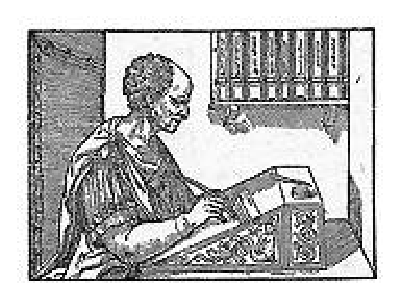
\includegraphics[width=0.5\linewidth]{lorem}
\captionof{figure}{\color{Green} Lorem.}
\end{center}\vspace{1cm}

\section{Experimentos/Resultados}

Fusce magna risus, molestie ut porttitor in, consectetur sed
mi. Vestibulum ante ipsum primis in faucibus orci luctus et ultrices
posuere cubilia Curae; Pellentesque consectetur blandit
pellentesque. Sed odio justo, viverra nec porttitor vel, lacinia a
nunc. Suspendisse pulvinar euismod arcu, sit amet accumsan enim
fermentum quis. 

\subsection*{Mathematical Section}

Nulla vel nisl sed mauris auctor mollis non sed. 

\begin{equation}
E = mc^{2}
\label{eqn:Einstein}
\end{equation}

Curabitur mi sem, pulvinar quis aliquam rutrum. (1) edf (2) ,
$\Omega=[-1,1]^3$, maecenas leo est, ornare at. $z=-1$ edf $z=1$ sed
interdum felis dapibus sem. $x$ set $y$ ytruem.  Turpis $j$ amet
accumsan enim $y$-lacina; ref $k$-viverra nec porttitor $x$-lacina.

Vestibulum ac diam a odio tempus congue. Vivamus id enim nisi:

\begin{eqnarray}
\cos\bar{\phi}_k Q_{j,k+1,t} + Q_{j,k+1,x}+\frac{\sin^2\bar{\phi}_k}{T\cos\bar{\phi}_k} Q_{j,k+1} &=&\nonumber\\ 
-\cos\phi_k Q_{j,k,t} + Q_{j,k,x}-\frac{\sin^2\phi_k}{T\cos\phi_k} Q_{j,k}\label{edgek}
\end{eqnarray}
and
\begin{eqnarray}
\cos\bar{\phi}_j Q_{j+1,k,t} + Q_{j+1,k,y}+\frac{\sin^2\bar{\phi}_j}{T\cos\bar{\phi}_j} Q_{j+1,k}&=&\nonumber \\
-\cos\phi_j Q_{j,k,t} + Q_{j,k,y}-\frac{\sin^2\phi_j}{T\cos\phi_j} Q_{j,k}.\label{edgej}
\end{eqnarray} 

Donec faucibus purus at tortor egestas eu fermentum dolor
facilisis. Maecenas tempor dui eu neque fringilla rutrum. Mauris
\emph{lobortis} nisl accumsan. Aenean vitae risus ante.
%

\vspace{1cm}
\begin{center}
\begin{tabular}{l l l}
\toprule
\textbf{Treatments} & \textbf{Response 1} & \textbf{Response 2}\\
\midrule
Treatment 1 & 0.0003262 & 0.562 \\
Treatment 2 & 0.0015681 & 0.910 \\
Treatment 3 & 0.0009271 & 0.296 \\
\bottomrule
\end{tabular}
\captionof{table}{\color{Green} Table caption}
\end{center}
\vspace{1cm}

Phasellus imperdiet, tortor vitae congue bibendum, felis enim sagittis
lorem, et volutpat ante orci sagittis mi. Morbi rutrum laoreet
semper. Morbi accumsan enim nec tortor consectetur non commodo nisi
sollicitudin. Proin sollicitudin. Pellentesque eget orci eros.

\section{Discussão}

O manual do \TeX~\cite{knuth1986} pode ser usado para aprendê-lo, e o livro do
Lamport~\cite{lamport1994} para aprender o \LaTeX, mas se quiser ir a fundo tem
que ver como o \TeX quero o os parágrafos em linhas~\cite{knuth1981}.

Two typesLorem ipsum dolor sit amet, consectetur adipiscing elit, sed
do eiusmod tempor incididunt ut labore et dolore magna aliqua. Uore eu
fugiat nulla pariatur.

\section{Conclusões}

\begin{itemize}
\item Pellentesque eget orci eros. Fusce ultricies, tellus et
  pellentesque fringilla.
\item Vestibulum sem ante, hendrerit a gravida ac, blandit quis magna.
\end{itemize}

\bibliographystyle{plain} % Plain referencing style
\bibliography{refs} % Use the example bibliography file %sample.bib

%----------------------------------------------------------------------------------------
%   AGRADECIMENTOS
%----------------------------------------------------------------------------------------
\section*{Agradecimentos}
\small \textnormal{This research was undertaken text is derived from
  sections 1.10.33 of Cicero's De finibus bonorum et malorumtext is
  derived from sections 1.10.33 of Cicero's De finibus bonorum et
  malorumtext is derived from sections 1.10.33 of Cicero's De finibus
  bonorum et malorum.}

\end{multicols}

\end{document}